% Source bitmap is unchanged; crop only its title and use the native frame title.
% 55bp at 144dpi removes 110px. Circle coordinates follow that viewport.
% Native square crops and circular clips retain the supplied portrait pixels.
\newcommand{\promptercoauthor}[3]{%
  \begin{scope}[shift={(#1,4.44)}]
    \begin{scope}
      \clip (0,0) circle[radius=.45cm];
      \node[inner sep=0pt] at (0,0)
        {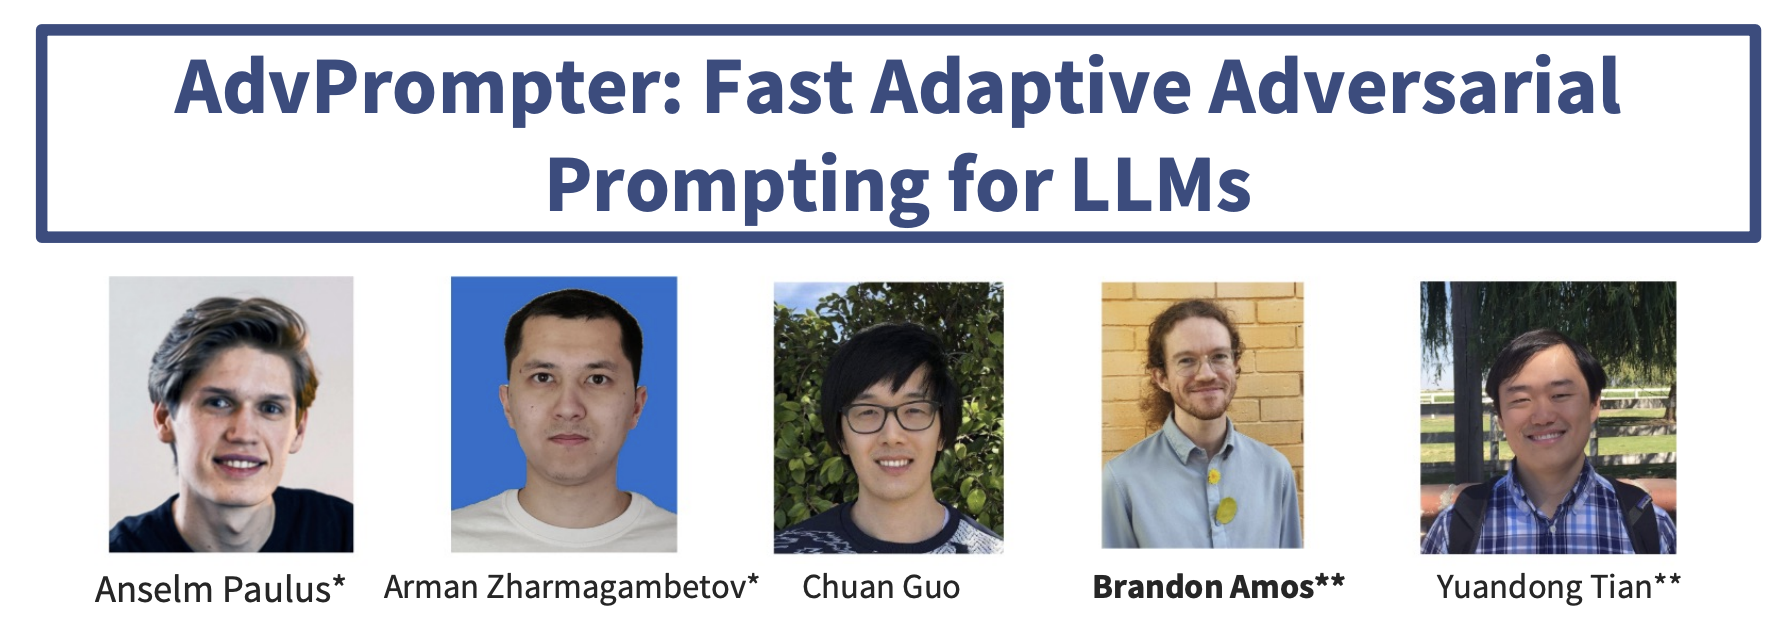
\includegraphics[trim=#2,clip,width=.9cm]{assets/advprompter-authors-source.png}};
    \end{scope}
    \draw[Muted!35,line width=.35pt] (0,0) circle[radius=.45cm];
  \end{scope}
  \node[anchor=north,align=center,text=Ink,font=\fontsize{8.5}{9.5}\selectfont,inner sep=0pt]
    at (#1,3.82) {#3};}
\newcommand{\jailbreakingtimeline}[1]{%
\begin{tikzpicture}
  \node[anchor=south west,inner sep=0pt] (timeline) at (0,0)
    {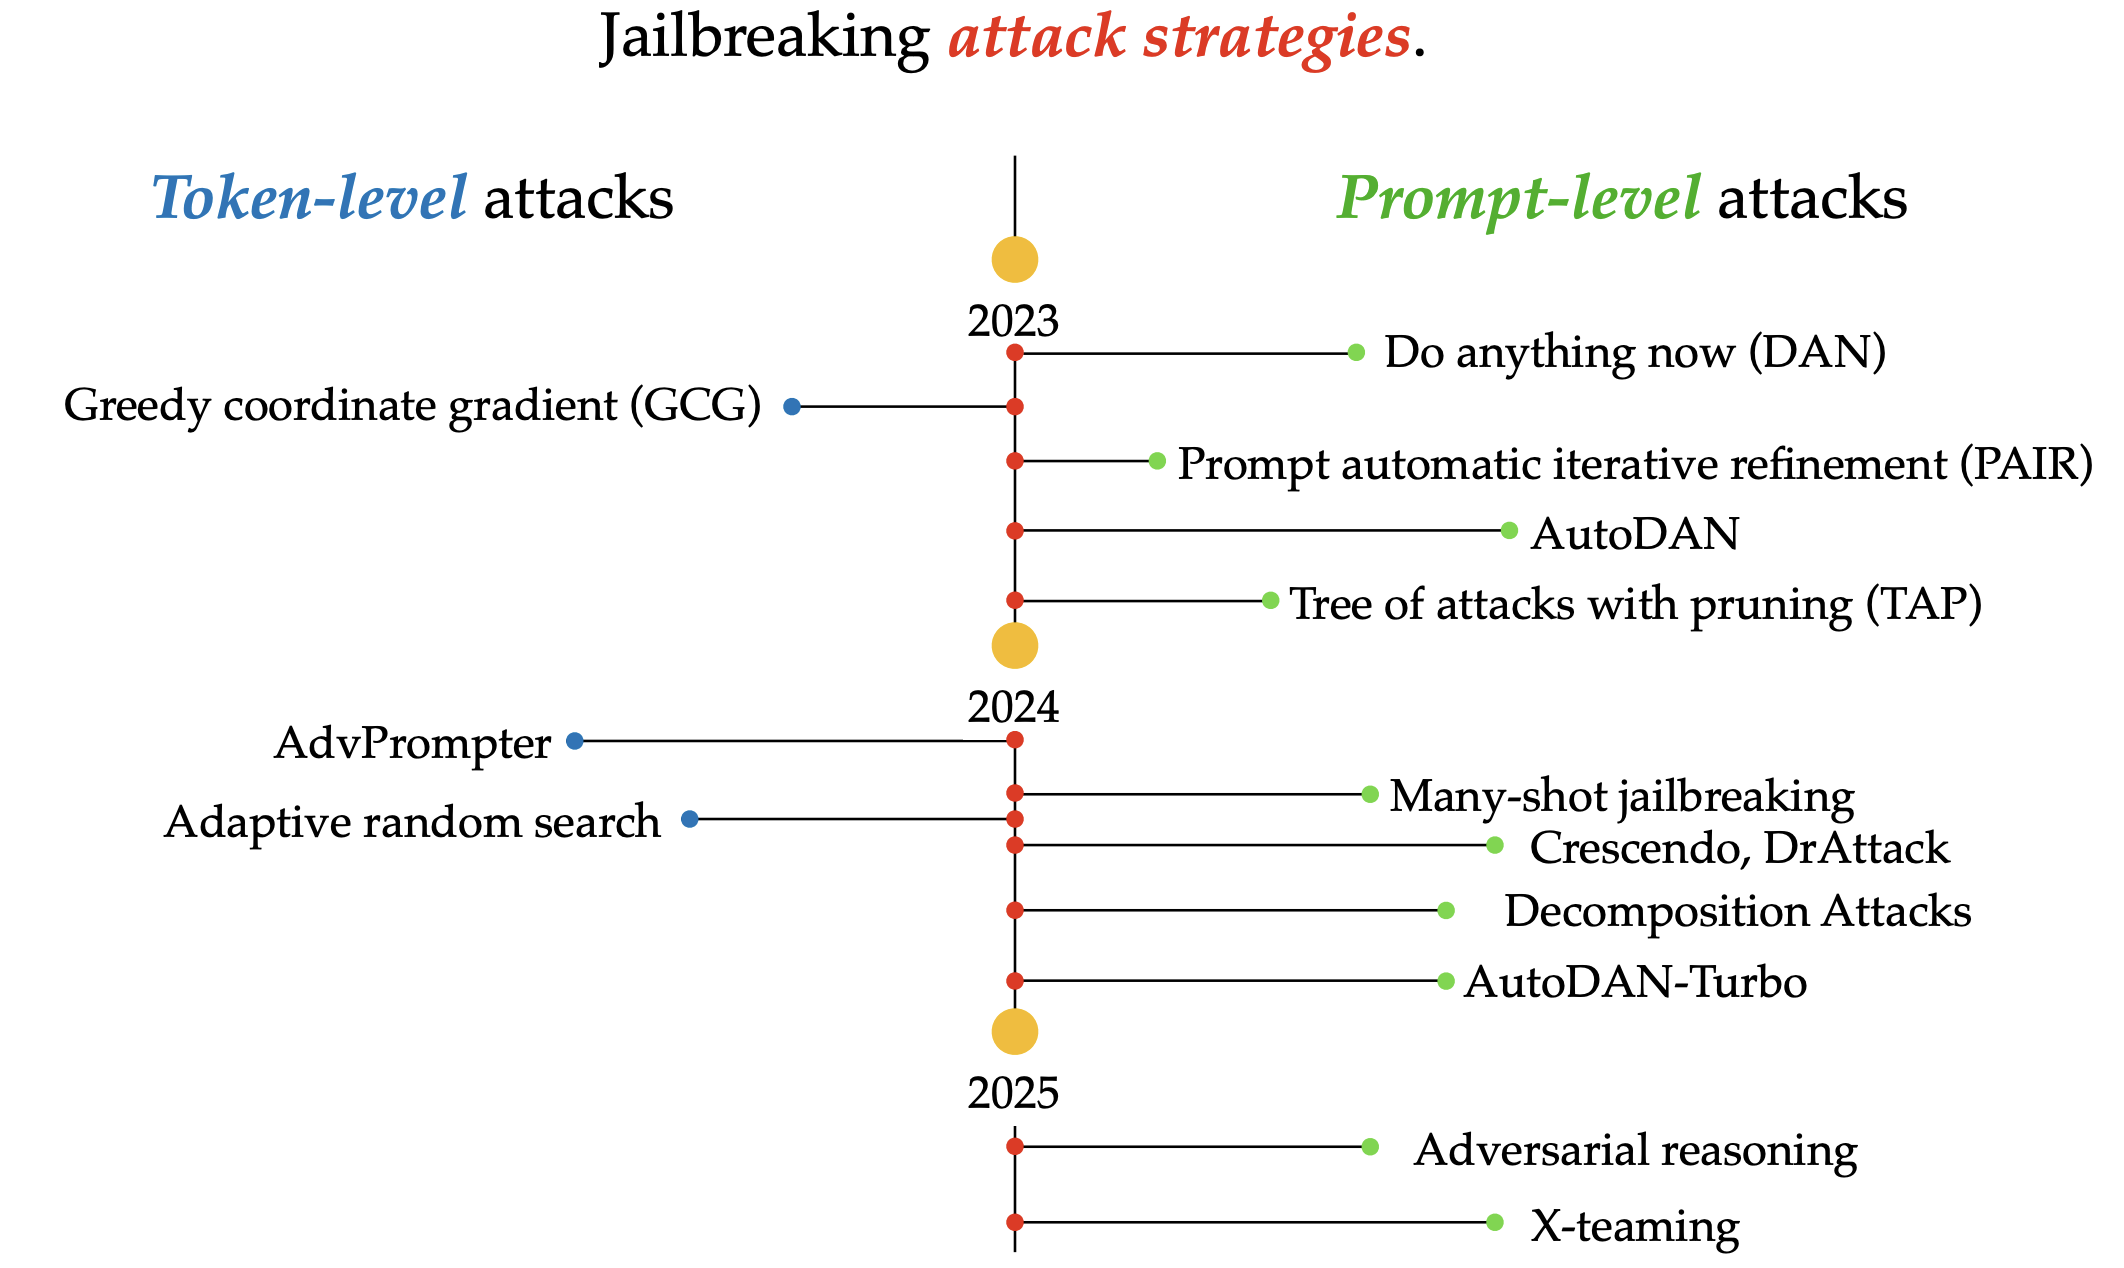
\includegraphics[height=5.6cm,trim=0 0 0 55bp,clip]{assets/icml2025-jailbreaking-timeline.png}};
  \ifnum#1>0
    \begin{scope}[x={(timeline.south east)},y={(timeline.north west)}]
      \draw[Accent,line width=1.4pt]
        (.198,.4544) ellipse[x radius=.085,y radius=.0460];
    \end{scope}
    % The callout deliberately overlays earlier timeline entries on this build.
    % Its overlay scope leaves the timeline, circle, and citation anchored.
    \begin{scope}[overlay]
      \draw[Accent,line width=1.4pt] (1.96,2.80) -- (1.96,3.10);
      \path[draw=Accent,fill=white,line width=1.4pt,rounded corners=3pt]
        (-.60,3.10) rectangle (10.85,5.98);
      \node[text=Muted,font=\fontsize{9}{11}\selectfont,inner sep=0pt] at (5.125,5.75)
        {ICML 2025};
      \node[anchor=north,align=center,text=Ink,font=\fontsize{11.5}{13.5}\selectfont,inner sep=0pt]
        at (5.125,5.48)
        {\href{https://proceedings.mlr.press/v267/paulus25a.html}{AdvPrompter: Fast Adaptive Adversarial Prompting for LLMs}};
      \promptercoauthor{.55}{54.5bp 42.5bp 708bp 146bp}{Anselm\\Paulus\authorcontribution{\ast}}
      \promptercoauthor{2.84}{225.5bp 52bp 546bp 145.5bp}{Arman\\Zharmagambetov\authorcontribution{\ast}}
      \promptercoauthor{5.13}{386.5bp 49bp 383bp 146.5bp}{Chuan\\Guo}
      \promptercoauthor{7.42}{543.5bp 56bp 233.5bp 147bp}{Brandon\\Amos\authorcontribution{\dagger}}
      \promptercoauthor{9.71}{710bp 42.5bp 47.5bp 141bp}{Yuandong\\Tian\authorcontribution{\dagger}}
    \end{scope}
  \fi
\end{tikzpicture}}
